\documentclass[a4paper,10pt]{book}

\usepackage[utf8]{inputenc}
\usepackage[T1]{fontenc}
\usepackage[francais]{babel}
\usepackage{lmodern}
\usepackage[top=3cm, bottom=3cm, left=4cm, right=2cm]{geometry}
\usepackage{amsmath}
\usepackage{amsfonts}
\usepackage{amsthm}
\usepackage{amssymb}
\usepackage{mathrsfs}
\usepackage{graphicx}
\usepackage{wrapfig}
\usepackage{stmaryrd}
\usepackage{calrsfs}
\usepackage{pdfpages}
\usepackage{url}
\usepackage{xlop}
\usepackage{multicol}
\usepackage{tikz}
\usepackage[pdftex, pdfauthor={Pierre Gimalac}, pdftitle={Algèbre et Analyse Élémentaire I}, pdfsubject={Mathématiques}, pdfkeywords={licence, mathématiques, informatique, fonctions, complexes, algèbre linéaire, propriétés de R, suites}, colorlinks=true, linkcolor=black, urlcolor=black]{hyperref}
\usepackage{chngpage}
\usepackage{pdflscape}

\newcommand{\R}{\mathbb{R}}
\newcommand{\Rpe}{\mathbb{R}_{+}^{*}}
\newcommand{\N}{\mathbb{N}}
\newcommand{\Z}{\mathbb{Z}}
\newcommand{\C}{\mathbb{C}}
\newcommand{\Q}{\mathbb{Q}}

\begin{document}

\begin{titlepage}
\newgeometry{margin=2.7cm}
\thispagestyle{empty}
\begin{center}
\vspace*{7cm}
\Huge \textsc{Algèbre et Analyse Élémentaire I}\\
\vspace{1.5cm}
\Large Pierre Gimalac\\
\vspace{0.5cm}
\large \textit{Licences de Mathématiques et d'Informatique}
\vfill
\end{center}
\large \textit{Septembre-Décembre 2016}
\hfill 
\large Cours de Régis de la Bretèche
\restoregeometry
\end{titlepage}

\renewcommand{\contentsname}{Sommaire}
\thispagestyle{empty}
\tableofcontents \thispagestyle{empty}
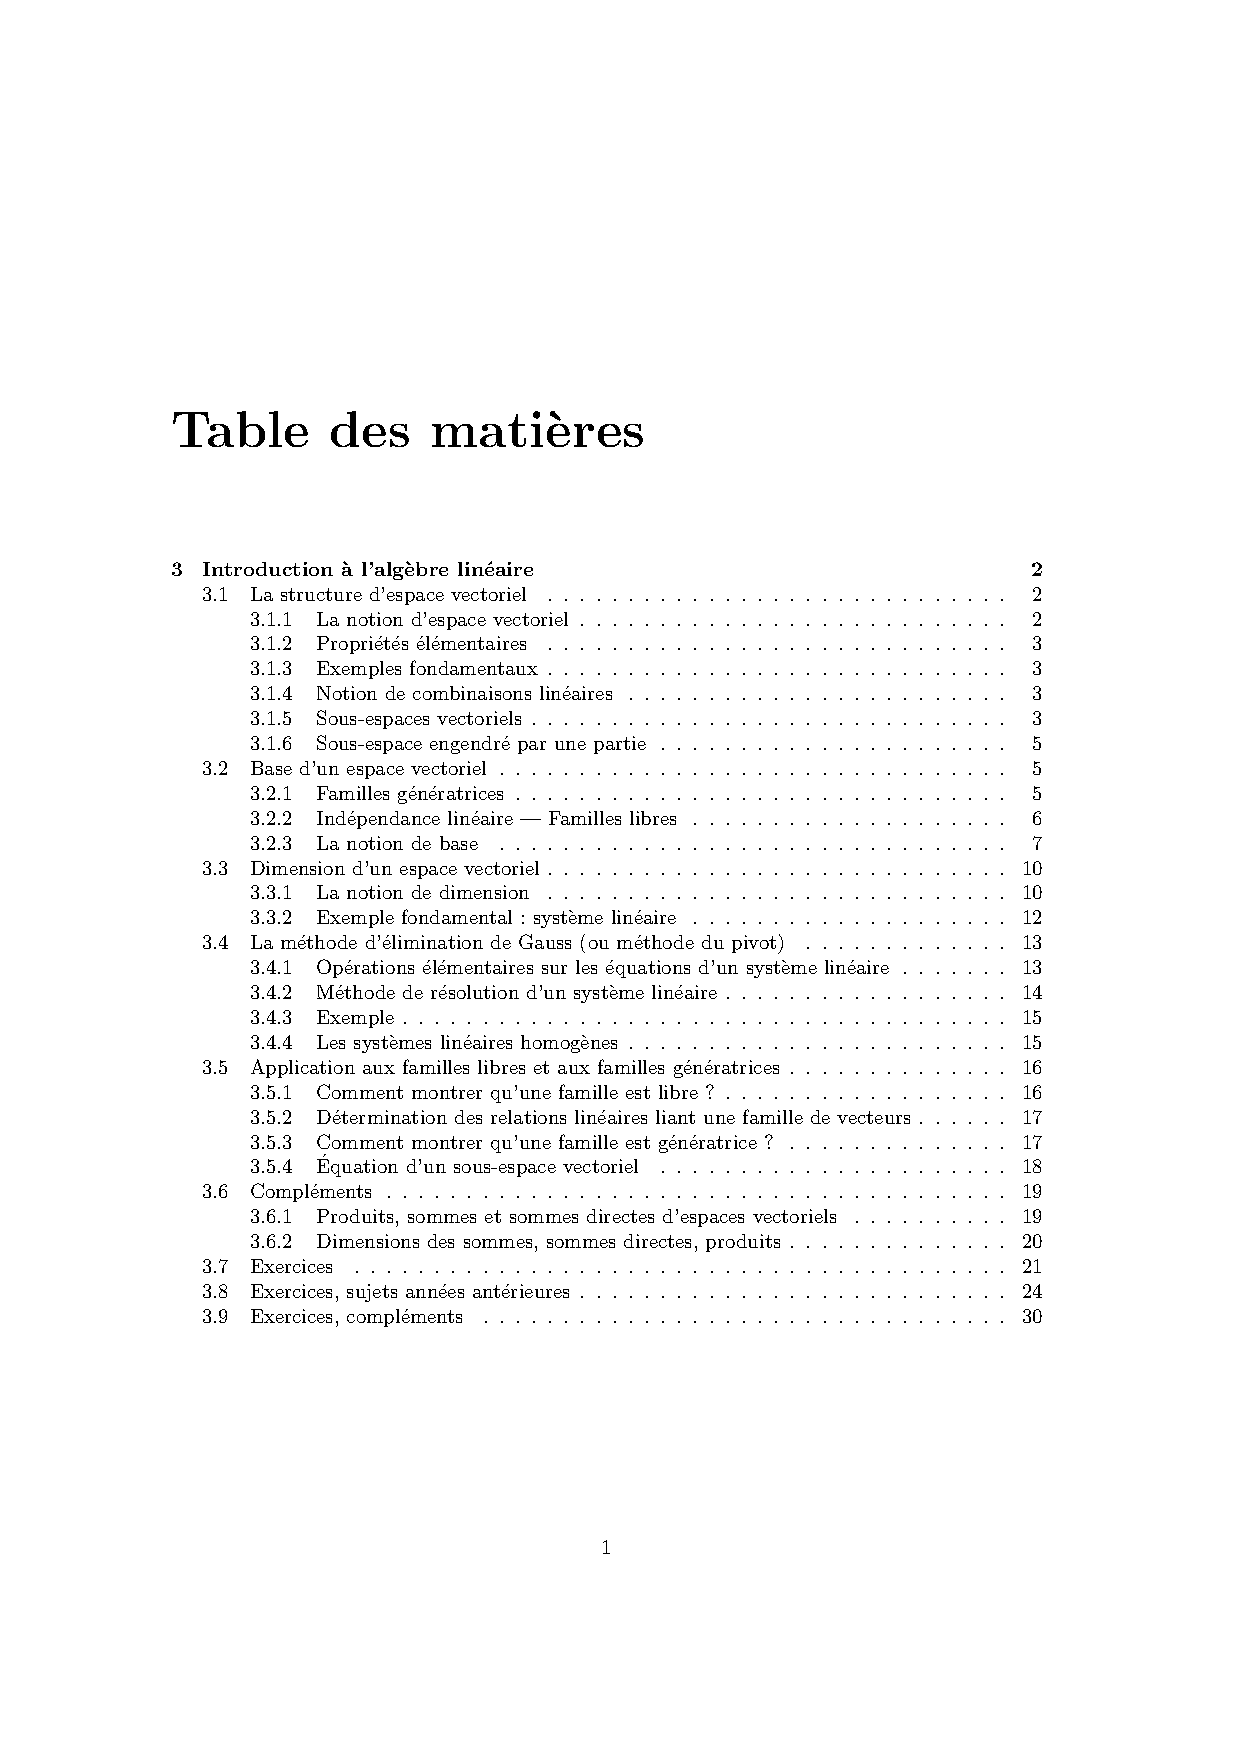
\includepdf[pages={1-2}]{images/Sommaires.pdf}

\chapter{Fonctions}

\section{Généralités}
\subsection{Application}
\subsubsection*{Définition}
Une application définie sur X et à valeur dans Y est une loi qui à tout élément de X associe un unique élément Y. \\
Si l'on note f cette application, l'élément associé à $x \in X$ par f est noté f(x). \\
X est l'ensemble de départ, Y est l'ensemble d'arrivée. \\
On note souvent \begin{displaymath}
f : \begin{array}{rcl}
X &\longrightarrow & Y \\
x &\longmapsto & y\end{array} \end{displaymath}
L'élément f(x) est l'image de x par f et x est un antécédent de f(x) par f.

\subsubsection*{Remarque :}
Une fonction peut être définie par son graphe : un graphe est un sous-ensemble $\Gamma$(f) de $X \times Y$ constitué par l'ensemble $\Gamma$=$\{(x;f(x))$, $\forall x \in X \}$.\\
De plus, si (x;y) et (x;y') $\in \Gamma ^{2}$, alors y=y' car un seul et unique élément de Y est associé à chaque élément de X.\\

\subsubsection{Exemples :}
\begin{itemize}\renewcommand{\labelitemi}{$\bullet$}
\item L'application identique $id_{X}$ d’un ensemble E dans lui-même est définie par $id_{X} (x) = x$ pour tout $x \in X$. Le graphe $\Gamma(id_{E}) = \{(x, x) | x \in X\}$ est la diagonale de $X^{2}$.
\item Si A est une partie de X, alors la restriction de $id_{X}$ à A s’appelle l’inclusion canonique
de A dans X.
\item L’application $pr_{1} : X \times Y \longrightarrow X$ définie par $pr_{1} (x,y) = x$ s’appelle la première projection de $X \times Y$ sur X. On définit de manière analogue la seconde projection $pr_{2} : X \times Y \longrightarrow Y$, $(x;y) \longrightarrow y$.
\item Soit X un ensemble. A une partie A de X on associe sa fonction caractéristique $\chi A : X \longrightarrow
\{0;1\}$, définie par $\chi A(x) = 1$ si $x \in A$ et $\chi A (x) = 0$ si $x \notin A$.
\item Soit $y \in Y$ un élément. L’application $\sigma_{y} : X \longrightarrow X \times Y$, définie par $\sigma_{y}(x) = (x;y)$ est appelée une section.
\item L’application $\lfloor\cdot\rfloor : \R \longrightarrow \Z$ qui au réel x associe le plus grand entier inférieur ou égal à x est appelée fonction partie entière. La partie entière $\lfloor x\rfloor$ de x est l’unique entier n tel que $n\leq x<n+1$.
La fonction partie entière est aussi notée $[x]$ ou $E(x)$ (ou $\lceil x\rceil$ dans le cas de l'entier supérieur).
\item Si X est un ensemble et $f : X \longrightarrow X$ est une application, on dit que $x \in X$ est invariant sous f si $f(x)=x$. L’ensemble des points invariants de f est donc donné par $\{x \in X | f(x)=x\}$.
\end{itemize}

\subsection{Composition de fonction}
Si f : $X \longrightarrow Y$ et g : $Y \longrightarrow Z$ sont deux applications, on peut définir la composée de f et g par \begin{displaymath} (g\circ f) : \begin{array}{rcl}
X &\longrightarrow & Z \\
x &\longmapsto & g(f(x))\end{array} \end{displaymath}

En général, $g\circ f \ne f\circ g$.\\

La composition des applications est associative:\\
$h : X \longrightarrow Y$, $g : Y \longrightarrow Z$, $f : Z \longrightarrow W$ alors $(f\circ g)\circ h=f\circ (g\circ h)$.\\

Une fonction d'une variable réelle à valeur réelle est une application de A dans $\mathbb{R}$ où $A \subset \mathbb{R}$.

\subsection{Monotonie}
Soit $f : X \longrightarrow Y$ une fonction et $I\subseteq X$. On dit que $\forall (x_{1},x_{2}) \in I^{2}$, f est :\\
\begin{itemize}\renewcommand{\labelitemi}{$\bullet$}
\item \emph{croissante} sur I si $(x_{1}<x_{2})\Longrightarrow (f(x_{1})\leq f(x_{2}))$.
\item \emph{strictement croissante} sur I si $(x_{1}<x_{2})\Longrightarrow (f(x_{1}) < f(x_{2}))$.
\item \emph{décroissante} sur I si $(x_{1}<x_{2})\Longrightarrow (f(x_{1})\geq f(x_{2}))$.
\item \emph{strictement décroissante} sur I si $(x_{1}<x_{2})\Longrightarrow (f(x_{1}) > f(x_{2}))$.
\item \emph{monotone} sur I si f est croissante ou décroissante.
\item \emph{strictement monotone} sur I si f est strictement croissante ou strictement décroissante.
\end{itemize}

\subsection{Parité}
Si le domaine de définition $D_{f}$ d'une fonction est symétrique par rapport à O,\\
($x \in D_{f}$ alors $-x \in D_{f}$) alors on dit que f est :
\begin{itemize}\renewcommand{\labelitemi}{$\bullet$}
\item paire, si $\forall x \in D_{f}, f(x)=f(-x)$
\item impaire, si $\forall x \in D_{f}, f(x)=-f(-x)$\\
\end{itemize}
On remarque que le graphe de f est symétrique à l'axe $O_{y}$ si et seulement si f est paire et est symétrique par la symétrie centrale de centre O si et seulement si f est impaire.\\

\subsection{Périodicité}
On dit qu'une fonction de $D_{f}$ dans $\mathbb{R}$ est périodique s'il existe T>0 tel que f(x+T)=f(x) pour tout $x \in D_{f}$.\\
Un tel nombre T est appelé la période de f s'il est le plus petit T>0 possible tel que f(x+T)=f(x) pour tout $x \in \mathbb{R}$.\\
\begin{figure}[h]
\begin{center}
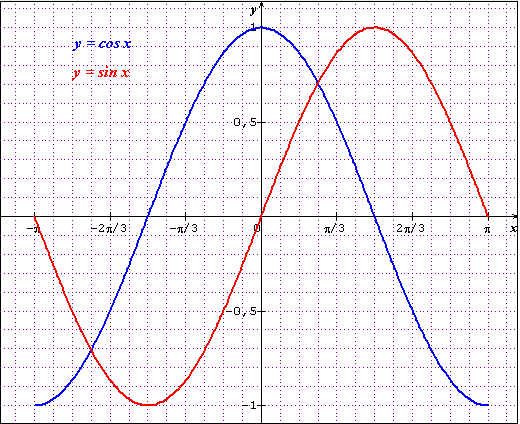
\includegraphics[scale=0.3]{images/001.png}
\caption{Les fonctions cosinus et sinus, fonctions périodiques respectivement paire et impaire}
\end{center}
\end{figure}

\subsection{Fonction injective, surjective et bijective}
\subsubsection{Ensembles de définition et image}
Soit $f: X \longrightarrow Y$ une application,\\
l'ensemble de définition de f est $D_{f}=\{x \in X : f(x) \text{est défini}\}$,\\
l'ensemble image de f est $Im_{f}=\{y \in Y : \exists x \in X, y=f(x) \}=\{f(x) : x \in X \}$.

\subsubsection{Injectivité}
Une application f : $X \longrightarrow Y$ est injective si $\forall (x;x')\in X^{2}$, $f(x)=f(x') \Leftrightarrow x=x'$.\\
Autrement dit si $f(x) \neq f(x')$ alors $x \neq x'$.\\
Chaque $y \in Y$ a au plus un seul antécédent.

\subsubsection{Surjectivité}
Une application $f : X \longrightarrow Y$ est surjective si et seulement si pour tout $y \in Y$, il existe au moins une valeur de x telle que y=f(x).\\
Il faut noter que cela dépend du choix de Y.\\
$f : D_{f} \longrightarrow f(D_{f})$ est une application surjective.

\subsubsection{Bijectivité}
Une application $f : X \longrightarrow Y$ est dite bijective si et seulement si elle est injective et surjective (donc si $\forall y \in Y$, $\exists$ $!$ $x \in X \mid f(x)=y$).\\
Toute fonction bijective est strictement monotone (et vice-versa).\\

\paragraph{} \textit{Bijection réciproque :} lorsque $f : X \longrightarrow Y$ est bijective, on peut définir sa bijection réciproque unique notée $f^{-1}$ qui vérifie \begin{displaymath} f^{-1} : 
\begin{array}{rcl}
Y &\longrightarrow & X\\
f(x) &\longrightarrow & x\\ \end{array}
\end{displaymath}

\subparagraph*{Propriétés}
\begin{enumerate}
\item $\forall (x ; y) \in X\times Y$, $(f^{-1} \circ f)(x)=f^{-1}(f(x))=x$ et $(f\circ f^{-1})(y)=y$.
\item Une fonction bijective est symétrique à sa bijection réciproque par la première diagonale.
\item Si $g\circ f$ est injective, alors f est injective.
\item Si $g\circ f$ est surjective, alors g est surjective.
\item Si g est injective et si $h : X \longrightarrow Y$ vérifie $g\circ f = g\circ h$, alors $f = h$.
\item Si f est surjective et si $h : Y \longrightarrow Z$ vérifie $g\circ f = h\circ f$, alors $g = h$.
\item Si f et g sont injectives, alors $g\circ f$ est injective.
\item Si f et g sont surjectives, alors $g\circ f$ est surjective.
\item Si f et g sont bijectives, alors $g\circ f$ est bijective et $(g\circ f )^{-1}= f^{-1}\circ g^{-1}$.
\item Une application de X dans Y est une bijection si et seulement si elle admet une bijection réciproque.\\

\emph{Démonstration :}\\
Supposons qu’il existe une application g telle que $g\circ f = id_{E}$ et $f\circ g= id_{F}$.\\
Puisque $id_{E} = g\circ f$ est injective, f est injective; de même, la surjectivité de $id_{F} = f\circ g$ entraîne la surjectivité de f. L’application f est donc bijective.
\end{enumerate}

\section{Fonctions logarithme et exponentielle}
\subsection{Fonction logarithme}
\subsubsection*{Définition}
On appelle logarithme népérien la fonction définie sur $\R _{+} ^{*}$ tel que $\ln (x)=\int _{1} ^{x} \dfrac{1}{t} dt$, ainsi $\ln(1)=0$.
$\ln(x)'=\dfrac{1}{x}$\\
$\ln(x)>0$ si $x>1$ et $\ln(x) <0$ si $x \in ]0 ;1[$.

\subsubsection*{Propriétés} 
La fonction $\ln : \R _{+} ^{*} \longrightarrow \R$ est strictement croissante, continue, indéfiniment dérivable \\et 
\begin{math} \begin{array}{rcl}
\underset{x \rightarrow 0^{+}}{\lim} ln(x)&=& -\infty \\
\underset{x \rightarrow +\infty}{\lim} ln(x) &=& +\infty \\
\end{array} \end{math}

De plus, la fonction $\ln$ est une bijection de $ \Rpe $ dans $\R$ et pour tout $(x ; y) \in  \Rpe {}^{2}$, $\ln(x\times y)=\ln(x)+\ln(y)$.\\

\textit{Démonstration}\\
Soit g tel que $g(x)=\ln(xy)-\ln(x)-\ln(y)$ avec y fixé, g est une fonction dérivable sur $\Rpe$\\
et $g'(x)=\frac{y}{xy}-\frac{1}{x}=0$ donc g est une fonction constante sur $\Rpe$,\\
or $g(1)=\ln(x)-\ln(x)-\ln(1)=0$ donc $\forall x \in \Rpe$, $g(x)=\ln(xy)-\ln(x)-\ln(y)$\\
d'où $\ln(xy)=\ln(x)+\ln(y)$.
\paragraph*{}\emph{Remarques :}\\ \\
$\forall x \in \Rpe , \ln(\frac{1}{x})=-\ln(x)$.\\ \\
On peut définir des fonctions logarithme en base a>0 noté $\log_{a}$ telle que $\log_{a}(x)=\frac{\ln(x)}{\ln(a)}$ d'où $log_{a}(a^{n})=n$.\\ \\
Souvent en info on utilise a=2, en sciences a=10.

\begin{figure}[h]
\begin{center}
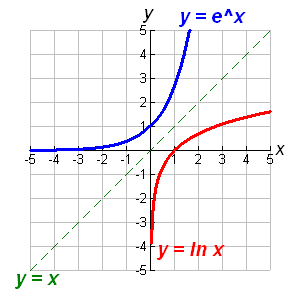
\includegraphics[scale=0.75]{images/003.png}
\caption{Fonctions logarithme népérien et exponentielle}
\end{center}
\end{figure}

\subsection{Fonction exponentielle}
\subsubsection{Définition}
La bijection réciproque de la fonction logarithme est l'exponentielle définie par $\exp : \R \longrightarrow \Rpe$.\\

\subsubsection{Propriétés}
La fonction exponentielle est croissante, indéfiniment dérivable, $\exp'(x)=\exp(x)$ et\\
\begin{math} \begin{array}{rcl}
\underset{x \rightarrow -\infty}{\lim} exp(x)&=& 0 \\
\underset{x \rightarrow +\infty}{\lim} exp(x)&=& +\infty \\\\\\
\end{array} \end{math}

De plus, la fonction $\exp$ est une bijection de $ \R $ dans $\Rpe$ et pour tout $(x ; y) \in  \R^{2}$,\\ $\exp(x+y)=\exp(x)\times\exp(y)$.\\

\subsubsection{Démonstration}
Soient $(x;y) \in \R^{2}$, comme $\ln$ est une bijection, $\exists$ $(u;v) \in \Rpe {}^{2}$ $|$ $x=\ln(u)$ et $y=\ln(v)$, d'où\\
$\exp(x)=\exp(\ln(u))=u$ et $\exp(y)=\exp(\ln(v))=v$ donc\\
$\exp(x+y)=\exp(\ln(u)+\ln(v))=\exp(\ln(u\times v))= u\times v =\exp(x)\times\exp(y)$\\

\subsubsection{Remarques}
L'axe $O_{x}$ est asymptote au graphe de exp et l'axe $O_{y}$ est asymptote au graphe de ln.\\\\
$\forall (n;x) \in \N \times \R$ , $x^{n}=exp(n\times\ln(x))$ car $ln(x^{n})=n\times\ln(x)$.\\\\
$\forall x \in \R$, $exp(x)=\sum\limits_{n=0}^{+\infty} \frac{x^{n}}{n!}$\\

\newpage
\subsection{Fonctions puissances}
Soit $\alpha \in \R$, on appelle fonction puissance la fonction définie par $f : \begin{array}{rcl} \Rpe &\longrightarrow &\Rpe\\
x &\longmapsto & x^{\alpha}=e^{\alpha ln(x)}\\ \end{array} $\\ \\
Si $\alpha \in \Z$, on peut étendre $D_{f}$ à $\R$ (tout en sachant que $0^{0}$ n'est pas défini).\\
Si $\alpha >0$, on peut étendre $D_{f}$ en 0 en prenant $f(0)=0$.

\begin{center}
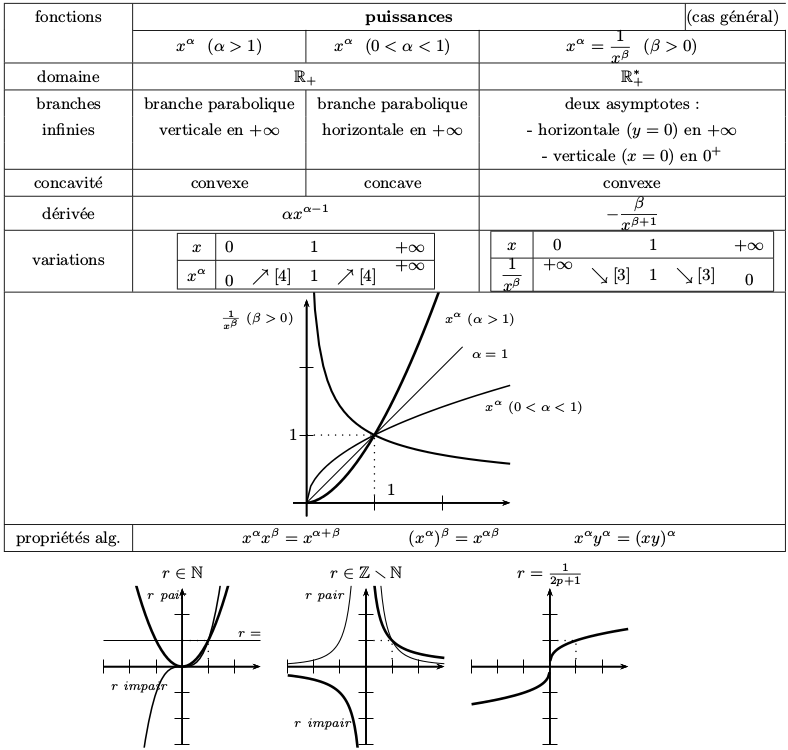
\includegraphics[scale=0.6]{images/005.png}
\end{center}

$\forall n \in \N^{*}$, on définit les fonctions racine n$^{ieme}$ par $x^{\frac{1}{n}}=exp(\frac{ln(x)}{n})=\sqrt[n]{x}$.\\

$f : x \longrightarrow x^{\alpha}$ avec $\alpha$ non nul est une bijection de $\Rpe$ dans $\Rpe$ dont la réciproque est $x \longrightarrow x^{\frac{1}{a}}$.\\\\

$(a^{x})'=(e^{ln(a)x})'=ln(a)\times a^{x}$
\newpage

\subsection{Le binôme de Newton} 
\begin{center} \begin{Large} $\forall (x;y)\in \C$, $n \in \N^{*}_{+}$, $(x+y)^{n}=\sum \limits_{k=0}^{n} \dbinom{n}{k} x^{k} y^{n-k}$ \end{Large} \end{center}

\subsubsection{Démonstration}
\emph{Prérequis : la formule du triangle de Pascal}\\

$\dbinom{n}{k-1}+\dbinom{n}{k}=\dbinom{n+1}{k}$\\\\

\textit{Démonstration :}\\
On sait que $\forall (k;n) \in \N^{2}$, $\dbinom{n}{k}=\frac{n!}{k!(n-k)!}$ d'où\\

\begin{large} $\begin{array}{rcl} \dbinom{n}{k-1}+\dbinom{n}{k} &=&\frac{n!}{(k-1)!(n-k+1)!}+\frac{n!}{k!(n-k)!}\\\\
&=&\frac{n!k}{k!(n+1-k)!}+\frac{n!(n+1-k)}{k!(n+1-k)!}\\\\
&=&\frac{n!(n+1)}{k!(n+1-k)!}\\\\
&=&\frac{(n+1)!}{k!(n+1-k)!}\\\\
\dbinom{n}{k-1}+\dbinom{n}{k}&=&\dbinom{n+1}{k} \end{array}$ \end{large}\\\\

\emph{Démonstration de la formule du binôme de Newton:}\\
On fait une récurrence sur $\N^{*}$: soit $P_{n}{}"(x+y)^{n}=\sum \limits_{k=0}^{n} \dbinom{n}{k} x^{k} y^{n-k}"$\\
Pour $n=1$, $(x+y)^{1}=x+y$ et $\sum \limits_{k=0}^{1} \dbinom{1}{k} x^{k} y^{1-k}=1*x*1+1*1*y=x+y$\\
donc $P_{1}$ est vraie.\\

Supposons que pour un entier naturel n quelconque, $P_{n}$ est vraie:\\\\
$\begin{array}{rcl} (x+y)^{n+1}&=&(x+y)\times \sum \limits_{k=0}^{n} \dbinom{n}{k} x^{k} y^{n-k}\\\\
&=&\sum \limits_{k=0}^{n} \dbinom{n}{k} x^{k+1} y^{n+1-(k+1)} + \sum \limits_{k=0}^{n} \dbinom{n}{k} x^{k} y^{n+1-k}\\\\
&=&\sum \limits_{k=1}^{n+1} \dbinom{n}{k-1} x^{k} y^{n+1-k}+ \sum \limits_{k=0}^{n} \dbinom{n}{k} x^{k} y^{n+1-k}\\\\
&=&x^{n+1}+y^{n+1}+\sum \limits_{k=1}^{n} (\dbinom{n}{k-1} + \dbinom{n}{k}) x^{k} y^{n+1-k}\\\\
&=&\sum \limits_{k=0}^{n+1} \dbinom{n+1}{k} x^{k} y^{n+1-k} \end{array}$\\\\

Ainsi $P_{n+1}$ est vraie donc $P_{n}$ est vraie pour tout $n \in \N^{*}$.

\section{Dérivées}
\subsection{Définition}
On considère I un intervalle ouvert de $\R$ et un point $x_{0} \in I$.\\
Soit $f : I \longrightarrow \R$ une fonction à valeurs réelles.
On dit que f est dérivable en $x_{0}$ si $\underset{x\rightarrow x_{0}}{lim} \frac{(f(x)-f(x_{0}))}{(x-x_{0})}$ existe.\\
Dans ce cas, on note cette limite $f'(x_{0})$ ou parfois $\frac{df(x_{0})}{dx}$.

\subsection{Propriétés}
Si l'on trace le graphe de f, la dérivée $f'(x_{0})$ s'interprète comme la pente de la droite tangente à la courbe au point $(x_{0};f(x_{0}))$.\\
L'équation de la tangente est $y-f(x_{0})=f'(x)(x-x_{0})$. Il s'agit du développement limité d'ordre 1 de f en $x_{0}$.\\ \\

h petit, $f(x_{0}+h)$ « ressemble » à $f(x_{0})+h\times f'(x_{0})$.\\

\emph{Variante :} il est parfois utile de définir les notions de dérivées à droite notée $\lim\limits_{\substack{x \rightarrow x_{0} \\ x>x_{0}}} \frac{f(x)-f(x_{0})}{x-x_{0}}$ et à gauche notée $\lim\limits_{\substack{x \rightarrow x_{0} \\ x<x_{0}}} \frac{f(x)-f(x_{0})}{x-x_{0}}$\\ \
\begin{figure}[h]
\begin{center}
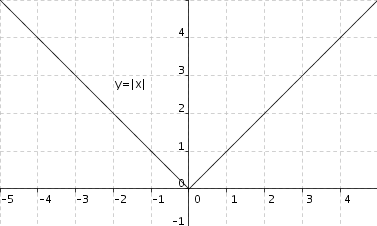
\includegraphics[scale=1]{images/004.png}
\caption{La dérivée de valeur absolue au point 0 n'est pas la même à gauche et à droite}
\end{center}
\end{figure}

\subsubsection*{Remarques}
Lorsque $\underset{x\rightarrow x_{0}}{lim} \frac{f(x)-f(x_{0})}{x-x_{0}} = +\infty$, on a une tangente verticale.\\ \\
Si f est dérivable, la fonction $x \longrightarrow f'(x)$ s'appelle la fonction dérivée.\\
Si f' est elle-même dérivable, sa dérivée s'appelle la dérivée seconde de f.\\
On introduit ainsi $f^{(n)}$ la dérivée n$^{ieme}$.\\
$f^{(n+1)}(x)=(f^{(n)})'(x)$

\newpage

\subsection{Fonctions usuelles}

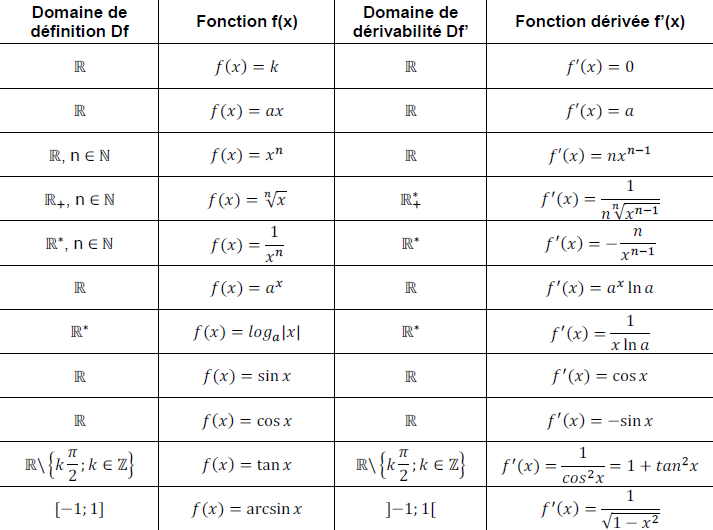
\includegraphics[scale=0.58]{images/017.png} \begin{figure}[h] \begin{center} \caption{Tableau des dérivées des fonctions usuelles} \end{center} \end{figure}

\textbf{Fonctions périodiques :} la dérivée d'une fonction de période T est périodique de période T.\\
$\forall x \in \R , f : f(x+T)=f(x)$ donc $f'(x+T)=f'(x)$.\\

\textbf{Fonctions paires et impaires :} la dérivée d'une fonction paire est impaire et vice-versa.\\ 
Si f est paire, $\forall x \in \R$, $f(-x)=f(x)$ donc $f'(-x)=-f'(-x)$. \\ \\

\begin{large} \emph{Digression} \end{large}\\ \\
Définition : une fonction $f : ]a;b[ \longrightarrow \R$ est dite n fois dérivable si elle possède des dérivées jusqu'à l'ordre n.\\ \\
Contre exemple:\\ \\
$f(x)=x\times |x|$\\
si x<0, $f(x)=-x^{2}$ et $f'(x)=-2x$\\
si x>0, $f(x)=x^{2}$ et $f'(x)=2x$\\
donc $f'(x)=2\times |x|$\\ \\
f est dérivable une fois mais pas deux.\\ \\

\subsection{Fonctions composées}
\label{Formules de dérivation}
\emph{Règle de calcul :} on considère f et g dérivables, alors $f+g$, $f \times g$, $f\circ g$ sont dérivables. En les points où g ne s'annule pas $\frac{f}{g}$ est dérivable.
\begin{enumerate}
\item $(f+g)'=f'+g'$
\item $(f\times g)'=f'\times g+f\times g'$
\item $(\frac{f}{g})'=\frac{(f'\times g-f\times g')}{g^{2}}$
\item $(f\circ g)'=g'*f'\circ g$
\item Si f admet une bijection réciproque et si $y_{0}=f(x_{0})$:\\
$(f^{-1})'(y_{0})=\frac{1}{f'(x_{0})}=\frac{1}{(f'\circ f^{-1})(y_{0})}$ \\
\end{enumerate}
\emph{Démonstration du 4 :}\\ \\
$\begin{array}{rcl}
(g\circ f)'(x)&=&\underset{h \rightarrow 0}{lim} \frac{(g\circ f)(x+h)-(g\circ f)(x)}{h}\\\\
&=&\underset{h \rightarrow 0}{lim} \frac{g(f(x+h))-(g(f(x))}{f(x+h)-f(x)}\times \frac{f(x+h)-f(x)}{h}\\\\
&=&g'(u(x))\times f'(x)\\
\end{array}$\\ \\ \\
\emph{Démonstration du 5 :}\\ \\
$\begin{array}{rcl}
(f^{-1})'(y_{0})&=&\underset{y \rightarrow y_{0}}{lim} \frac{f^{-1}(y)-f^{-1}(y_{0})}{y-y_{0}}\\\\
\text{or } \frac{f^{-1}(y)-f^{-1}(y_{0})}{y-y_{0}}&=&\frac{f^{-1}(y)-f^{-1}(y_{0})}{f(f^{-1}(y))-f(f^{-1}(y_{0}))}\\\\
&=&\frac{1}{\frac{f(f^{-1}(y))-f(f^{-1}(y_{0}))}{f^{-1}(y)-f^{-1}(y_{0})}}\\\\
\text{donc } (f^{-1})'(y_{0})&=&\underset{y \rightarrow y_{0}}{lim} \frac{f^{-1}(y)-f^{-1}(y_{0})}{y-y_{0}}\\\\
&=&\frac{1}{f'(f^{-1}(y_{0}))}\\\\\\
\end{array}$

\subsection{Sens de variation et signe de la dérivée}
Soit $f : X \longrightarrow Y$ une fonction définie et dérivable sur $I \subseteq \R$, alors si f' la dérivée de f est telle que pour tout $x \in I$, f'(x)
\begin{itemize}\renewcommand{\labelitemi}{$\bullet$}
\item est positif, f est croissante.
\item est strictement positif, f est strictement croissante.
\item est négatif, f est décroissante.
\item est strictement négatif, f est strictement décroissante.
\item est nul, f est constante.\\
\end{itemize}
f admet un extremum local en $x_{0}$ si et seulement si $\exists$ $x_{0} \in I$ | f' s'annule et change de signe en $x_{0}$.

\newpage

\subsection{Formule de Leibniz}
Soient f et g deux fonctions n fois dérivables alors $f\times g$ est n fois dérivable et \\\\ \begin{Large}
$(f\times g)^{(n)} = \sum \limits_{k=0}^{n} \dbinom{n}{k}\times f^{(k)}\times g^{(n-k)}$\end{Large} \\\\\\\\
\textbf{Démonstration}\\\\\\
Démontrons la formule par récurrence sur $\N$.\\ \\
n=1 évident:\\ \\
$\begin{array}{rcl}
(fg)^{(1)}&=&\sum \limits_{k=0}^{1} \dbinom{1}{k} \times f^{(k)}\times g^{(1-k)} \\\\
&=& fg'+f'g
\end{array}$
\\ \\ \\ \\
Partons de la formule à l'ordre n : \\ \\
$\begin{array}{rcl}
\text{On a } (fg)^{(n)}&=&\sum \limits_{k=0}^{n} \dbinom{n}{k}\times f^{(k)}\times g^{(n-k)}\\\\
(fg)^{(n+1)}=((fg)^{(n)})' &=&\sum \limits_{k=0}^{n} \dbinom{n}{k} \times (f^{(k+1)}\times g^{(n-k)}+f^{(k)}\times g^{(n+1-k)})\\\\
&=&\sum \limits_{k=0}^{n} \dbinom{n}{k} \times f^{(k+1)}\times g^{(n+1-(k+1))}+\sum \limits_{k=0}^{n} \dbinom{n}{k} \times f^{(k)}\times g^{(n+1-k)}\\\\
&=&\sum \limits_{k=1}^{n+1} \dbinom{n}{k-1} \times f^{(k)}\times g^{(n+1-k)}+\sum \limits_{k=0}^{n} \dbinom{n}{k} \times f^{(k)}\times g^{(n+1-k)}\\\\
&=&\sum \limits_{k=1}^{n} \dbinom{n}{k-1}f^{(k)}g^{(n+1-k)}+\sum \limits_{k=1}^{n} \dbinom{n}{k}f^{(k)}g^{(n+1-k)}+f^{(n+1)}g+fg^{(n+1)}\\\\
&=&\sum \limits_{k=0}^{n}{}(\dbinom{n}{k}+\dbinom{n}{k-1})\times f^{(k)}g^{(n+1-k)}+f^{(n+1)}g^{(0)}+f^{(0)}g^{(n+1)}\\\\
\end{array}$ \\ \\
Or, $\forall k \in \{0;...;n\}$, la formule du triangle de Pascal est : $\dbinom{n}{k}+\dbinom{n}{k-1}=\dbinom{n+1}{k}$\\\\
Donc $(fg)^{(n+1)}=\sum \limits_{k=0}^{n+1}{}\dbinom{n+1}{k}\times f^{(k)}\times g^{(n+1-k)}$
\\\\\\
Nous obtenons bien la formule au rang n+1. Un raisonnement par récurrence permet donc de conclure.\\

\newpage

\section{Fonctions trigonométriques}
\subsection{Fonctions cosinus et sinus}
\begin{figure}[!h] \begin{center}
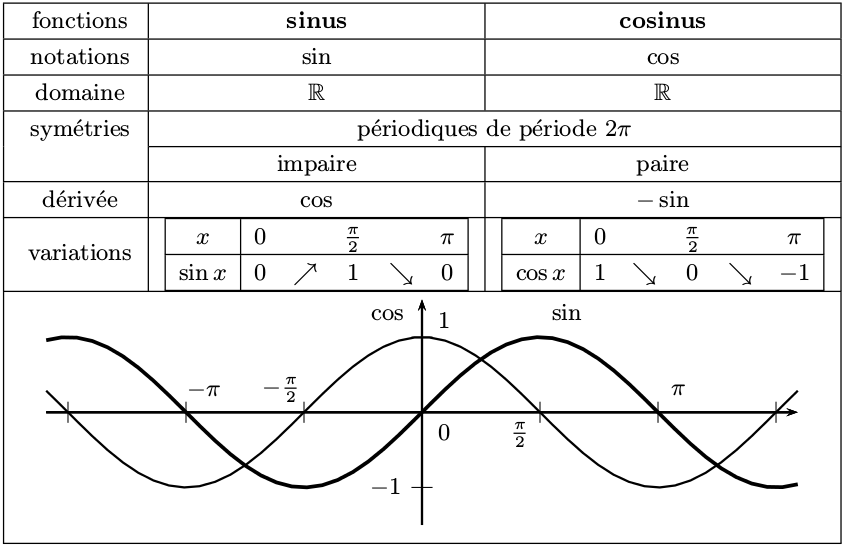
\includegraphics[scale=0.524]{images/010.png}
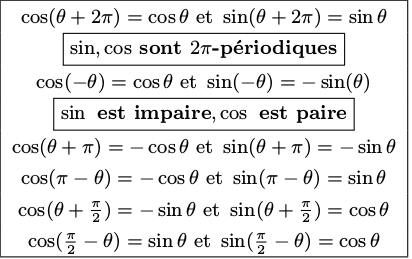
\includegraphics[scale=0.7]{images/013.png}
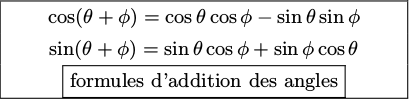
\includegraphics[scale=0.7]{images/011.png}
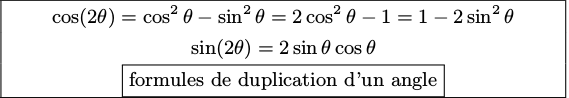
\includegraphics[scale=0.7]{images/012.png}
\end{center} \end{figure}

\newpage
\subsection{Fonctions tangente}
\begin{center}
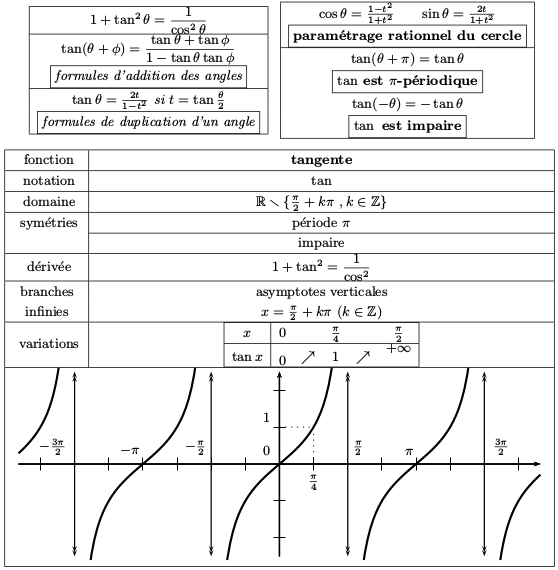
\includegraphics[scale=0.78]{images/009.png}
\end{center}

\subsection{Valeurs remarquables}
\emph{Pour plus de détails, voir page \pageref{Cercle trigo}.}
\begin{center}
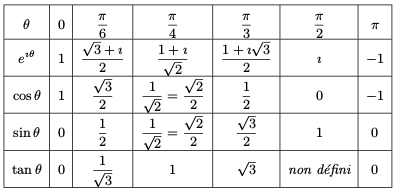
\includegraphics[scale=0.75]{images/007.png}
\end{center}
\newpage

\section*{Fonctions réciproques}
\subsection{Fonction Arcsin}
La fonction $\sin : [-\frac{\pi}{2} ; \frac{\pi}{2}] \longrightarrow [-1;1]$ est une bijection. Sa bijection réciproque se note Arcsin.

\subsubsection{Propriétés}
La fonction $Arcsin : [-1;1] \longrightarrow [-\frac{\pi}{2} ; \frac{\pi}{2}]$ est continue, croissante, impaire et indéfiniment dérivable sur $]-1;1[$.\\
$y=Arcsin(x) \Leftrightarrow x=sin(y)$ ET $y \in [-\frac{\pi}{2} ; \frac{\pi}{2}]$.\\\\
Grâce à la formule de la dérivée de la fonction réciproque (\ref{Formules de dérivation}), on a $(Arcsin)'(x)=\frac{1}{\sqrt{1-x^{2}}}$.

\begin{wrapfigure}[16]{r}{6cm} 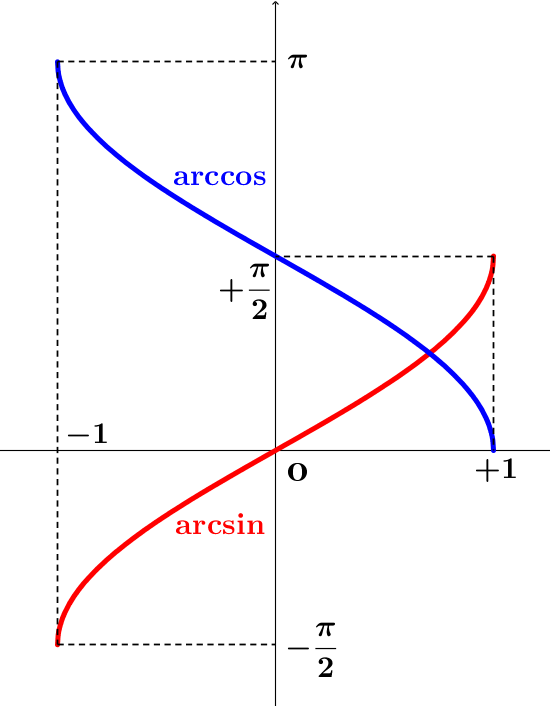
\includegraphics[scale=1.5]{images/015.png} \end{wrapfigure}
\subsection{Fonction Arccos}
La fonction $cos : [0 ; \pi] \longrightarrow [-1;1]$ est une bijection. Sa bijection réciproque se note Arccos.

\subsubsection{Propriété}
La fonction $Arccos : [-1;1] \longrightarrow [0 ; \pi]$ est continue, positive, décroissante.\\ \\
Toutes les propriétés de l'Arccos se déduisent de celles de l'Arcsin grâce à la formule :\\
$\forall x \in [-1;1]$, $Arcsin(x)+Arccos(x)=\frac{\pi}{2}$.\\\\
\emph{Démonstration :}\\
$sin(\frac{\pi}{2}-Arccos(x))=cos(Arccos(x))=x$ \\
donc $\frac{\pi}{2}-Arccos(x)=Arcsin(x)$.\\

Arcsin(sin(x)) ne vaut pas toujours x car si $x \notin [-\frac{\pi}{2} ; \frac{\pi}{2}]$, $Arcsin(sin(x)) \neq x$.\\
En revanche, $\forall x \in [-1;1]$, $sin(Arcsin(x))=x$.\\ \\ \\

\subsection{Fonction Arctan}
La fonction tangente une bijection de $\frac{\pi}{2} +k\pi$, $k \in \Z$ dans $\R$. Sa bijection réciproque se note $Arctan : \R \longrightarrow ]-\frac{\pi}{2};\frac{\pi}{2}[$.\\

$tan'(x)=\frac{1}{cos^{2}(x)}=tan^{2}(x)+1$ donc Arctan est dérivable et \\
$Arctan'(x)=\frac{1}{tan^{2}(Arctan(x))+1}=\frac{1}{x^{2}+1}$
\begin{center} 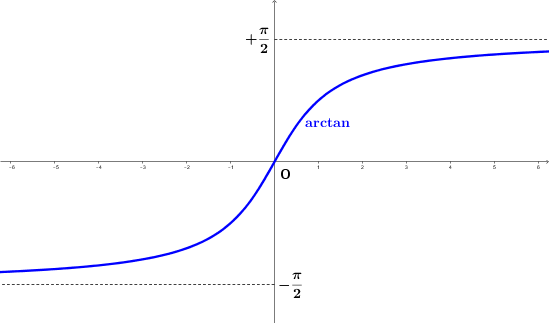
\includegraphics[scale=1.5]{images/018.png} \end{center}

\section{Fonctions hyperboliques}
\begin{center} 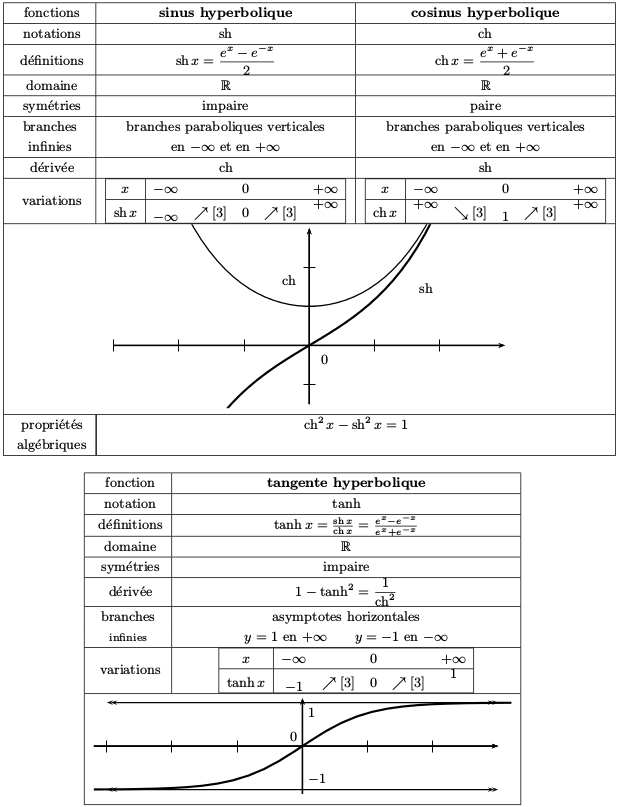
\includegraphics[scale=0.75]{images/022.png} \end{center}

\newpage

\section{Autres notions}
\subsection{Limites}
Soit $f : X \longrightarrow Y$, $x_{0} \in X$ et $y_{0} \in Y$.\\

\textit{Limite réelle en un réel}\\
On dit que f tend vers $y_{0}$ lorsque x tend vers $x_{0}$ et on écrit $\underset{x \rightarrow x_{0}}{\lim}=y_{0}$\\
si $\forall \epsilon >0$, $\exists \alpha >0$, $\forall x \in X\backslash \{x_{0}\}$, $|x-x_{0}|<\alpha \Longrightarrow |f(x)-y_{0}|<\epsilon$.\\

Ce qui signifie que l'on peut rendre $|f(x)-y_{0}|$ (la distance entre $f(x)$ et $y_{0}$) aussi petite que l'on veut, pourvu qu'on choisisse x dans X, différent de $x_{0}$, mais suffisamment proche de $x_{0}$.\\

\textit{Limite infinie en un réel}\\
On dit que f tend vers $+\infty$ lorsque x tend vers $x_{0}$ et on écrit $\lim\limits_{\substack{x \rightarrow x_{0} \\ x \in X}} f(x)=+\infty$ si\\
$\forall \epsilon >0$, $\exists \alpha >0$, $\forall x \in X\backslash \{x_{0}\}$, $|x-x_{0}|<\alpha \Longrightarrow f(x)>\epsilon$.\\

\textit{Limite finie en l'infini}\\
Si f(x) est défini quand x tend vers l'infini ($Y=]a;+\infty[$ avec $a \in \R$), alors on dit que f tend vers $y_{0}$ lorsque x tend vers l'infini et on écrit $\underset{x \rightarrow + \infty}{\lim} f(x)=y_{0}$ si\\
$\forall \epsilon >0$, $\exists \alpha >0$, $\forall x>a$, $x>\alpha \Longrightarrow |f(x)-y_{0}|<\epsilon$.\\

\textit{Limite infinie en l'infini}\\
Si f(x) est défini quand x tend vers l'infini ($Y=]a;+\infty[$ avec $a \in \R$), alors on dit que f tend vers $+\infty$ lorsque x tend vers l'infini et on écrit $\underset{x \rightarrow + \infty}{\lim} f(x)=+\infty$ si\\
$\forall \epsilon >0$, $\exists \alpha >0$, $\forall x>a$, $x>\alpha \Longrightarrow f(x)>\epsilon$.\\
\begin{center}
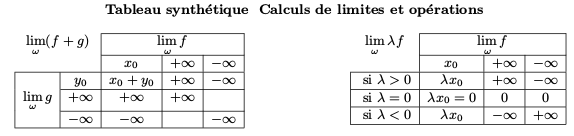
\includegraphics[scale=0.675]{images/024.png}
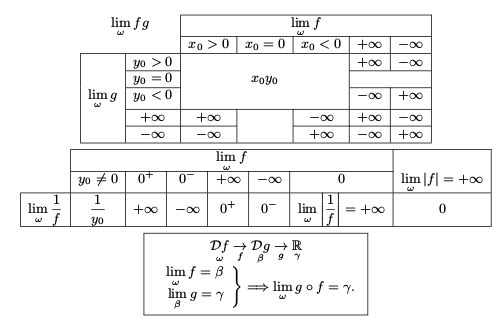
\includegraphics[scale=0.725]{images/023.png}
\end{center}

\subsection{Concavité et convexité}
On considère $f: d_{f} \longrightarrow \R $, $I \subset D_{f}$ un intervalle.\\

On dit que f est convexe sur I si les cordes de f sont au dessus de sa courbe représentative.\\
$\forall (x;y) \in I^{2}$, $\forall t \in [0;1]
f(tx+(1-t)y) \leqslant tf(x)+(1-t)f(y)$\\

De même, on dit que f est concave si les cordes de f sont au dessous de sa courbe représentative.\\
$\forall (x;y) \in I^{2}$, $\forall t \in [0;1]$, $f(tx+(1-t)y) \geqslant tf(x)+(1-t)f(y)$\\

Soit f une fonction 2 fois dérivable sur I telle que $f''(x)\geqslant 0$, $\forall x \in I$, alors f est convexe sur I.

Soit f une fonction 2 fois dérivable sur I telle que $f''(x)\leqslant 0$, $\forall x \in I$, alors f est concave sur I.
\begin{figure}[!h] \begin{center} 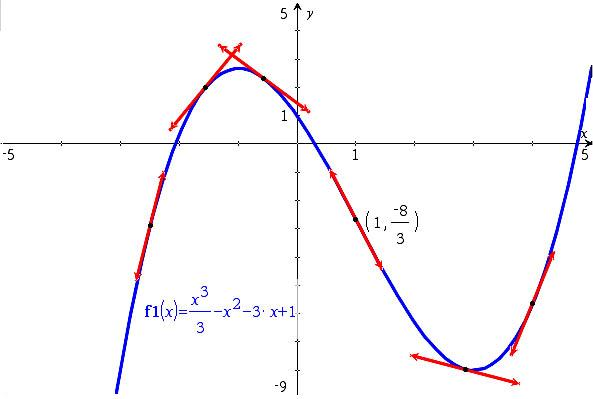
\includegraphics[scale=0.6]{images/016.jpg} \caption{Cette fonction est concave jusqu'en 1, son point d'inflexion, puis convexe} \end{center} \end{figure}

\subsection{Asymptotes}
Soit $f : X \longrightarrow Y$ une fonction, $x_{0} \in X$ et $y_{0} \in Y$.\\

\textit{Asymptote verticale}\\
Si $\underset{x \rightarrow x_{0}}{\lim} f(x)=\pm\infty$\\
alors la droite d'équation $x=x_{0}$ est asymptote au graphe de f en $x_{0}$.\\

\textit{Asymptote horizontale}\\
Si f(x) est défini quand x tend vers l'infini et $\underset{x \rightarrow \pm\infty}{\lim} f(x)=y_{0}$\\
alors la droite d'équation $y=y_{0}$ est asymptote au graphe de f en $+\infty$.\\

\textit{Asymptote oblique}\\
Si f(x) est défini quand x tend vers l'infini et s'il existe $(a;b) \in \R^{2}$ $|$ $\underset{x \rightarrow \pm\infty}{lim} f(x)-ax=b$\\
alors la droite d'équation $y=ax+b$ est asymptote au graphe de f en $\pm\infty$.\\\\

\emph{Méthode pour déterminer l’existence d'une asymptote oblique en l'infini :}\\\\
Si $\underset{x\rightarrow \pm\infty}{lim} \frac{f(x)}{x}=a$ (avec $a \in \R$), on étudie la limite de $f(x)-ax$,\\
alors si $\underset{x\rightarrow \pm\infty}{lim} f(x)-ax=b$ (avec $b \in \R$),\\
f admet une asymptote oblique d'équation $ax+b$ en l'infini.

\subsection{Translation et dilatation}
Soit c>0. Pour déterminer le graphe de la fonction g(x) dans les cas suivants, il faut effectuer les opérations suivantes sur le graphe de f :\\ \begin{enumerate}
\item Si $g(x)=f(x)+c$ il faut translater le graphe de f (x) de c unités vers le haut.
\item Si $g(x)=f(x)-c$ il faut translater le graphe de f (x) de c unités vers le bas.\\
\begin{figure}[h] \begin{center} 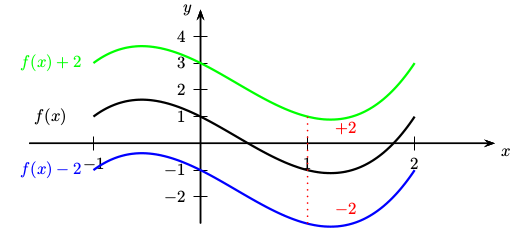
\includegraphics[scale=0.5]{images/019.png} \caption{Graphe de la fonction $f(x)=x^{3}-x^{2}-2x+1$ et des fonctions $f(x)+2$ et $f(x)-2$} \end{center} \end{figure}
\item Si $g(x)=f(x-c)$ il faut translater le graphe de f (x) de c unités vers la droite.
\item Si $g(x)=f(x+c)$ il faut translater le graphe y de f (x) de c unités vers la gauche.
\begin{figure}[h] \begin{center} 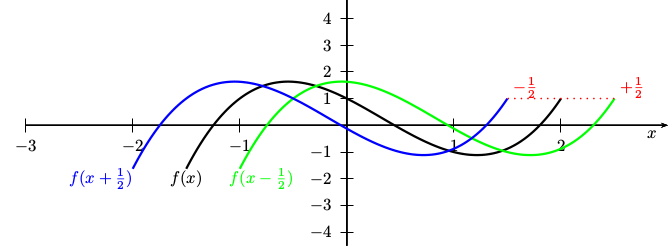
\includegraphics[scale=0.5]{images/020.png} \caption{Graphe de la fonction $f(x)=x^{3}-x^{2}-2x+1$ et des fonctions $f(x-\frac{1}{2})$ et $f(x+\frac{1}{2})$} \end{center} \end{figure}
\item Si $g(x)=c*f(x)$ il faut dilater verticalement le graphe de f (x) d’un facteur c.
\item Si $g(x)=f(cx)$ il faut dilater horizontalement le graphe de f (x) d’un facteur $\frac{1}{c}$.
\begin{figure}[h] \begin{center} 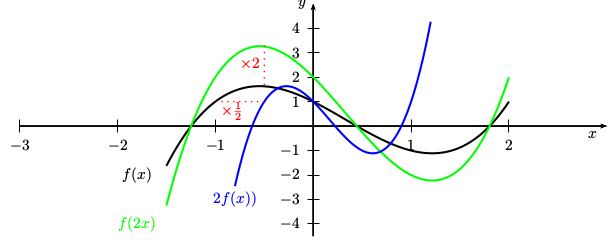
\includegraphics[scale=0.5]{images/021.png} \caption{Graphe de la fonction $f(x)=x^{3}-x^{2}-2x+1$ et des fonctions $2f(x)$ et $f(2x)$} \end{center} \end{figure}
\end{enumerate}

\subsection{Continuité}
Soit f une fonction définie de I dans $\R$ et $x_{0} \in I$, on dit que f est continue en $x_{0}$ si et seulement si $\lim_{x \rightarrow x_{0}}=f(x_{0})$.\\
La continuité est une notion locale: on parle de continuité de f en un point de I.\\

$\forall \epsilon >0$, $\exists$ $\alpha >0$, $\forall x \in I$, $|x-x_{0}|<\alpha \Longrightarrow |f(x)-f(x_{0})|<\epsilon$

\subsubsection{Propriétés}
Soient f et g deux fonctions définies de I dans $\R$, continue en $x_{0}$, \\
alors $f+g$, $f-g$, $f\times g$ sont continues en $x_{0}$. Si $g(x_{0}) \neq 0$, $\frac{f}{g}$ est continue en $x_{0}$.\\ \\
Si $g : I \longrightarrow J$ est continue en $x_{0}$ et $f : J \longrightarrow \R$ est définie en $y_{0}=f(x_{0})$ alors $f\circ g$ est continue en $x_{0}$.

\subsubsection{Théorème}
Si une fonction f est dérivable en un point $x_{0}$ de son ensemble de définition, alors elle est continue en ce point $x_{0}$.\\
La réciproque de ce théorème est fausse.

\subsubsection{Théorème des valeurs intermédiaires}
Soient a et b deux réels avec a<b Soit $f : [a;b] \longrightarrow \R$ une fonction continue. Si $f(a)<c$ et $f(b)>c$, alors il existe $\xi \in ]a;b[$ tel que $f(\xi)=c$.\\

\textit{Démonstration}\\
Par translation, en considérant la fonction $x \longrightarrow f(x)-c$ au lieu de f, on se ramène au cas où $c=0$.\\\\
L’ensemble $X=\{x \in [a;b]$ $|$ $f(x)<0\}$ est non vide (car $a \in X$) et majoré par b. Il admet donc une borne supérieure : $\xi=sup(X)$. Montrons que $\xi$ répond à la question et vérifie $f(\xi)=0$.\\\\
Par l’absurde supposons que $f(\xi)=\kappa <0$ et prenons $\epsilon =-\frac{\kappa}{2}>0$. La continuité de f en $\xi$ garantie l’existence de $\delta >0$ tel que :\\

$|f(x)-\kappa |<\frac{\kappa}{2}$ si $|x-\xi |<\delta$ de sorte que $f(x)>\frac{\kappa}{2}>0$ si $\xi -\delta <x<\xi$\\\\
ce qui est impossible puisqu'alors $\xi -\delta$ serait un majorant de X et $\xi$ est le\\ plus petit majorant de X.\\

Supposons à présent $f(\xi)=\kappa <0$ et prenons $\epsilon =-\frac{\kappa}{2}>0$. La continuité de f en $\xi$ garantie l’existence de $\delta >0$ tel que $|f(x)-\kappa |<\frac{\kappa}{2}$ si $|x-\xi |<\delta$\\\\
de sorte que $f(x)<\frac{\kappa}{2}<0$ si $\xi <x<\xi +\delta$ ce qui est impossible par définition de $\xi =sup(X)$.
\begin{center} 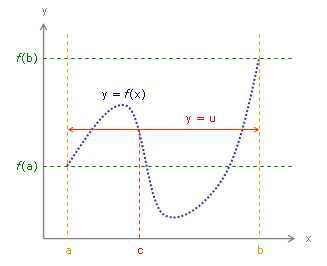
\includegraphics[scale=0.525]{images/025.png} \end{center}

\chapter{Nombres Complexes}
\section{Introduction}

Dans $\R$, l'équation $x^{2}=-1$ n'a pas de solution. Pour résoudre cela,\\on introduit une quantité i qui vérifie $i^{2}=-1$.\\

\subsection{Définition}
Un nombre complexe z s'écrit $z=x+i \times y$ ou $x \in \R$, $y \in \R$. Il s'agit de la forme algébrique d'un nombre complexe.\\ \\
Cet ensemble de nombres est noté $\C$, il est en bijection avec $\R \times \R$. \\

On dit que x est la \textit{partie réelle} de z et y est la \textit{partie imaginaire} de z.

On note $\Re(z)$ la partie réelle de z et $\Im(z)$ sa partie imaginaire.\\

On dit que z est un réel si $\Im(z)=0$ et un imaginaire pur si $\Re(z)=0$.

\subsection{Opérations dans $\C$}


\subsubsection{La somme}
On définit la somme de deux complexes $z=x+iy$ et $z'=x'+iy'$\\
comme $z+z'=x+x'+i(y+y')$.\\

\subsubsection{Le produit}
On définit également le produit de deux complexes $z=x+iy$ et $z'=x'+iy'$\\
comme $zz'=(xx'-yy')+i(xx'+yy')$.\\\\

\emph{Propriétés du produit dans $\C$ :}\\ \\
Le produit est une loi: \begin{itemize}\renewcommand{\labelitemi}{$\bullet$}
\item commutative : $zz'=z'z$
\item associative : $(zz')z''=z(z'z")$
\item distributive par rapport à l'addition : $z"(z+z')=z"z+z"z'$.\\
\end{itemize}


\section{Nombre conjugué}
\subsection{Définition}
Le conjugué d'un complexe $z=x+iy$ est noté $\overline{z}$ et $\overline{z}=x-iy$.\\

\subsection{Propriétés de la conjugaison}

\begin{itemize}\renewcommand{\labelitemi}{$\bullet$}
\item $\overline{z+z'}=\overline{z}+\overline{z'}$\\
\item $\overline{zz'}=\overline{z} \times \overline{z'}$\\
\item $\forall \lambda \in \R$, $ \in \C$, $\overline{\lambda z}=\lambda \overline{z}$ \\
\item La conjugaison est involutive: $\overline{\overline{z}}=z$.
\end{itemize}

\section{Autres notations}
\subsection{Représentation graphique}
Dans le plan $(O;\vec{i};\vec{j})$, on représente z un nombre complexe par le point $M_{z}$ de coordonnées $(x;y)$.

\subsubsection{Module}
Le module r de z est noté $|z|$ et $|z|=\sqrt{x^{2}+y^{2}}=\sqrt{z \overline{z}}$.\\
Dans le plan $(O;\vec{i};\vec{j})$, $|z|=OM_{z}$.\\

\subsubsection{Argument}
L'argument $\theta$ de z est noté $arg(z)$ et est déterminé à $2\pi$ près.\\
Dans le plan $(O;\vec{i};\vec{j})$, $\theta =(\vec{i};\overset{\longrightarrow}{OM_{z}})$.\\

\subsubsection{Coordonnées polaires}
On appelle $(|z|;Arg(z))=(r;\theta)$ les coordonnées polaires de z.\\
\begin{figure}[h] \begin{center}
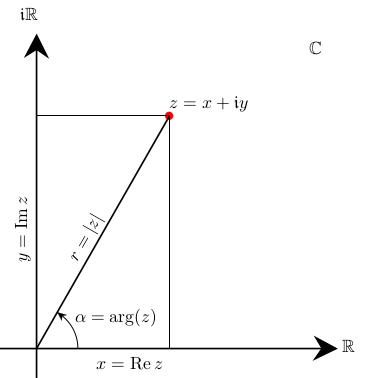
\includegraphics[scale=0.4]{images/201.png}
\caption{Représentation graphique d'un complexe}
\end{center} \end{figure}

\subsection{Forme trigonométrique}

Tout complexe z peut s'écrire sous la forme $z=r[cos(\theta)+i\times sin(\theta)]$ \\où $r=|z|$ et $\theta \equiv Arg(z) (2\pi)$.\\

\subsubsection{Propriétés :}
\begin{enumerate} 
\item $r[cos(\theta)+i\times sin(\theta)]=r'[cos(\theta ')+i\times sin(\theta ')]$ avec $r,r' \geq 0$ \\
si et seulement si $r=r'$ et $\theta \equiv \theta '(2\pi)$
\item $|\overline{z}|=|z|$
\item $arg(zz')\equiv arg(z)+arg(z') (2\pi)$
\item $Arg(\overline{z}) \equiv -Arg(z) (2\pi)$.\end{enumerate}

\subsubsection{Démonstrations :}
\begin{enumerate}
\item $z=z' \Leftrightarrow$
$\left \{ \begin{array}{rcl} OM&=&OM' \\
(\vec{i};\overset{\longrightarrow}{OM})&=&(\vec{i};\overset{\longrightarrow}{OM'}) \end{array} \right .
\Leftrightarrow$
$\left \{ \begin{array}{rcl} |z|=r&=&r' \\
\theta &\equiv &\theta '(2\pi) \end{array} \right .$\\
\item $|\overline{z}|=\sqrt{x^{2}+(-y)^{2}}=|z|$\\
\item $zz'=rr'*[cos(\theta)cos(\theta ')-sin(\theta ')sin(\theta ')+i(sin(\theta)cos(\theta ')+cos(\theta)sin(\theta')]$\\
$zz'=rr'[cos(\theta +\theta ')+isin(\theta +\theta ')]$ \\
donc $Arg(zz')\equiv \theta +\theta ' (2\pi)$\\
\item $\overline{z}=r[cos(\theta)-isin(\theta)]=r[cos(-\theta)+isin(-\theta)]$\\
donc $Arg(\overline{z})\equiv -\theta (2\pi)$\\
\end{enumerate}

\subsection{Forme exponentielle}
\subsubsection{Définition}
On pose $e^{i\theta}=cos(\theta)+i\times sin(\theta)$, et plus généralement $e^{x+iy}=e^{x}[cos(y)+isin(y)]$.\\\\
On a donc $e^{i\theta}=\sum\limits_{n=0}^{+\infty} \frac{(i\theta)^{n}}{n!}$.

\subsubsection{Propriétés}
\begin{enumerate}
\item Tout nombre complexe non nul peut s'écrire sous la forme $z=e^{z'}$ où $z' \in \C$.
\item $e^{z}=e^{z'} \Leftrightarrow \left \{ \begin{array}{rcl} Re(z)&=&Re(z')\\
Im(z)&=&Im(z') (2\pi) \end{array} \right .$\\
\item $e^{z+z'}=e^{z}\times e^{z'}$
\item $e^{\overline{z}}=e^{z}$
\end{enumerate}

\subsubsection{Démonstrations}
\begin{enumerate}
\item On écrit $z=re^{i\theta} =e^{ln(r)+i\theta}=e^{z'}$ avec $z'=ln(r)+i\theta$.
\item $e^{z}=e^{z'} \Leftrightarrow Re(z)+i\times Im(z)=Re(z')+i\times Im(z') \Leftrightarrow \left \{ \begin{array}{rcl} Re(z)&=&Re(z')\\
Im(z)&=&Im(z') (2\pi) \end{array} \right .$\\
\item $e^{z+z'}=e^{x+iy+x'+iy'}=e^{x+x'}\times [cos(y+y')+i\times sin(y+y')]=e^{x}\times e^{x'} \times (e^{iy}+e^{iy'})=e^{z}\times e^{z'}$
\item $e^{\overline{z}}=e^{x-iy}=e^{x}\times [cos(-y)+i\times sin(-y)]=e^{x}\times [cos(y)-i\times sin(y)]=e^{z}$\\\\
\end{enumerate}

\section{Propriétés des nombres complexes}
\begin{enumerate}
\item Tout nombre complexe z$ \neq 0$ admet un inverse  $z^{-1}=\frac{\overline{z}}{|z|^{2}}=\frac{x-iy}{x^{2}+y^{2}}$\\
car $zz'=|z|^{2} \Leftrightarrow \frac{z\overline{z}}{|z|^{2}}=1$.\\
\item $\forall z \in \C$, $z=x+iy$, $\left \{ \begin{array}{rcl} x&=&\frac{z+\overline{z}}{2} \\
y&=&\frac{z-\overline{z}}{2i} \end{array} \right . $\\
\item $\forall z \in \C$, $z' \in \C$, $|zz'|=|z| \times |z'|$.\\
\item Une inégalité triangulaire pour les complexes: $|z+z'|\leq |z|+|z'|$
\begin{figure}[h] \begin{center}
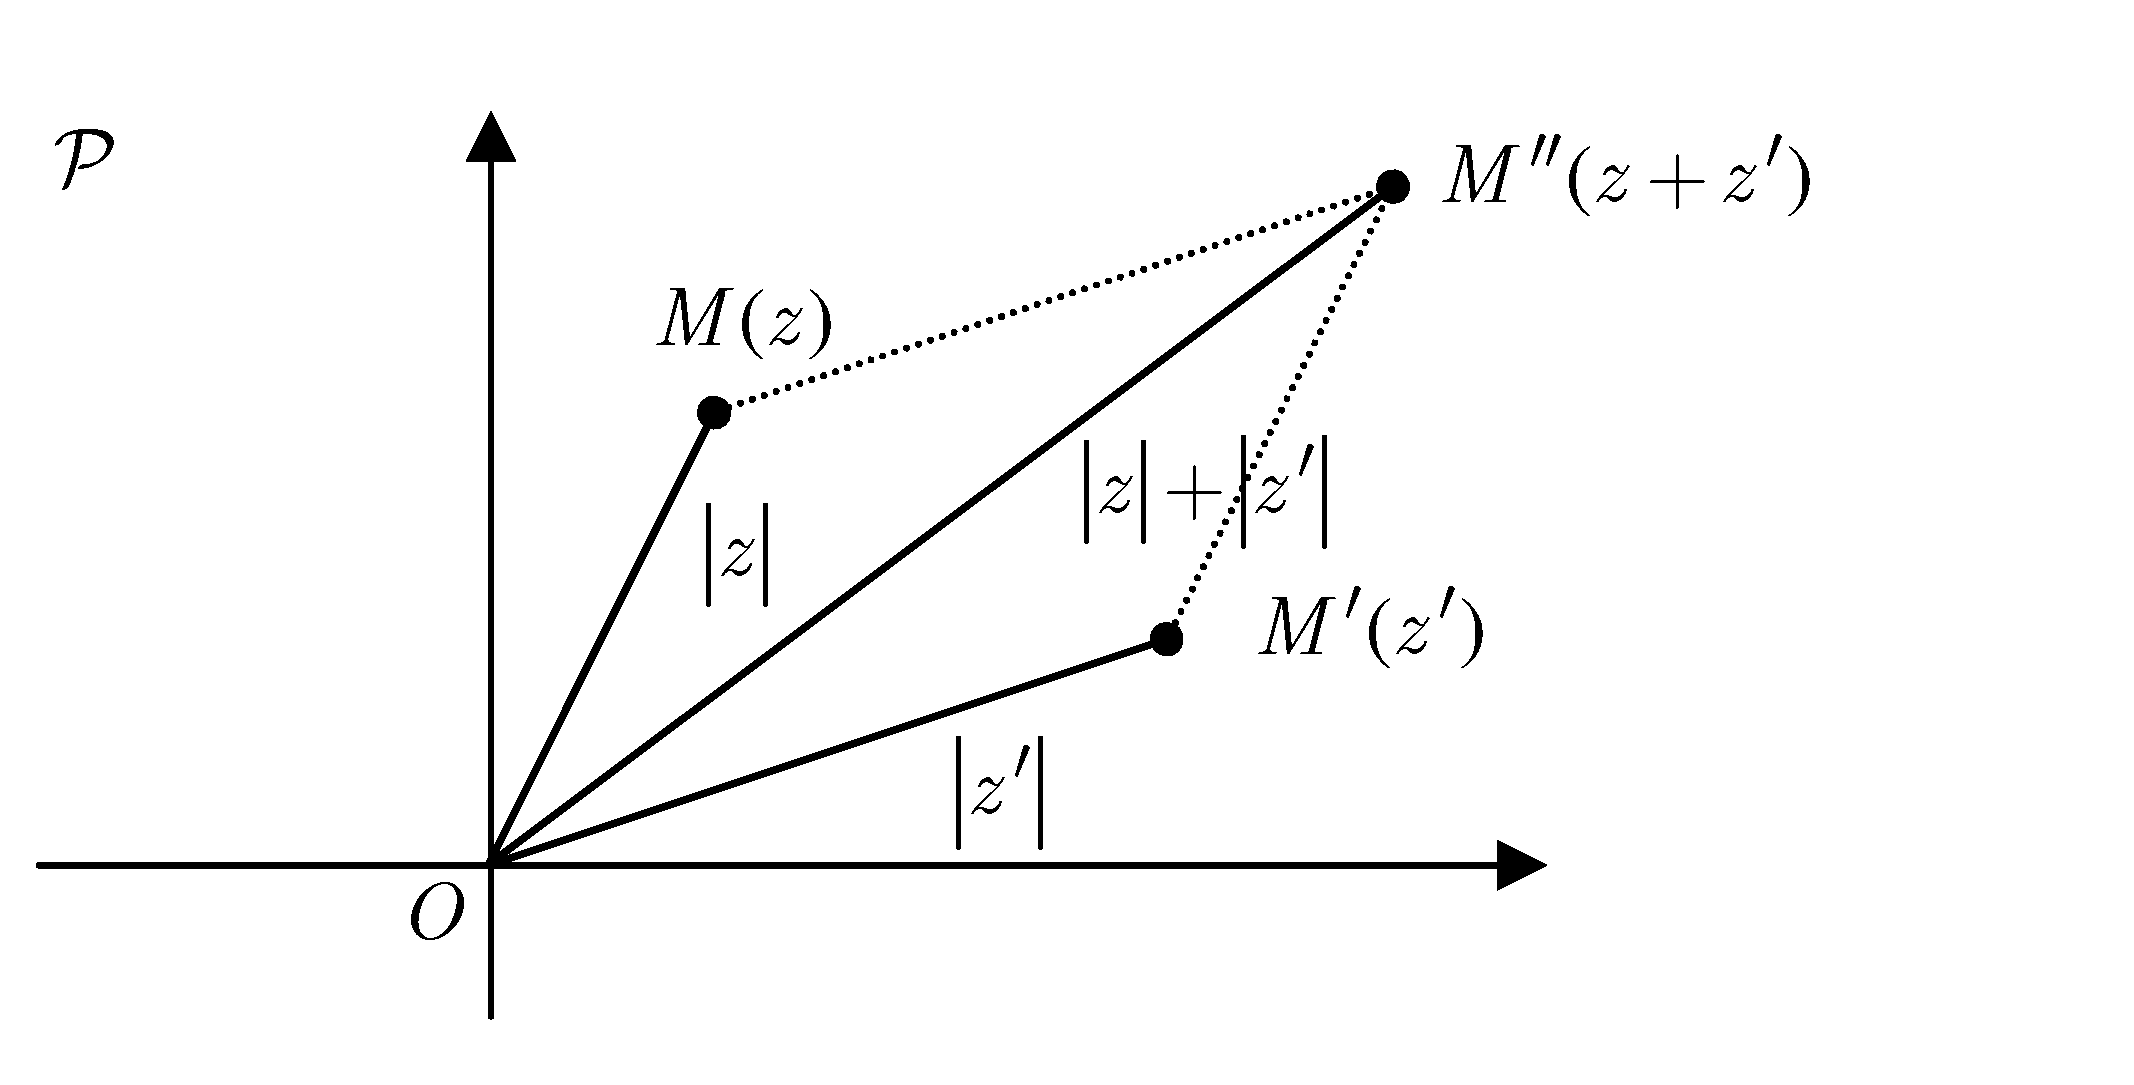
\includegraphics[scale=1.1]{images/200.png}
\caption{Représentation graphique de l'inégalité triangulaire}
\end{center} \end{figure}
\subsubsection{Démonstration}
$|z+z'|^{2}-(|z|+|z'|)^{2} = z\overline{z}+z\overline{z'}+\overline{z}z'+z'\overline{z'}-|z|^{2}-|z'|^{2}-2|zz'| \\
|z+z'|^{2}-(|z|+|z'|)^{2}=2\times Re(z\overline{z'})-2|zz'|$\\\\
donc $|z+z'|^{2}-(|z|+|z'|)^{2} \leq 0$\\\\
d'où $|z+z'|^{2}\leq(|z|+|z'|)^{2}$ et donc $|z+z'| \leq |z| + |z'|$.\\
\item $arg(zz')=arg(z)+arg(z')$ et $|zz'|=|z|\times |z'|$.
\begin{figure}[h] \begin{center}
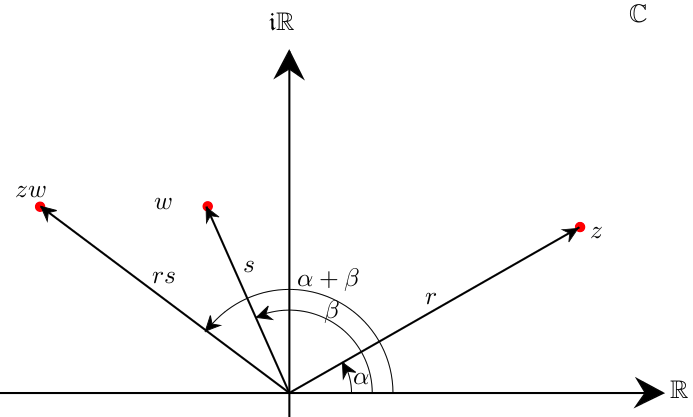
\includegraphics[scale=0.375]{images/203.png}
\caption{Représentation graphique de la multiplication de complexes}
\end{center} \end{figure}
\end{enumerate}

\section{Résolution d'équations dans $\C$}
\subsection{Théorème de d'Alembert-Gauss}
\textit{Théorème fondamental de l'algèbre}\\\\
Soit P un polynôme non constant à coefficient dans $\C$ alors $\exists$ $\alpha \in \C$ tel que $P(\alpha)=0$.\\\\
Tout polynôme P peut s’écrire sous la forme $P(x)=a_{0}(x-\alpha_{1})...(x-\alpha_{d})$
où $a_{0} \in \C^{*}$ et $\alpha_{i} \in \C$ (non nécessairement distinctes), donc un polynôme de degré $n\in\N$ admet n racines complexes pouvant être multiples.

\subsection{Racines n$^{iemes}$}
\subsubsection{Définition}
Soient $z \in \C$* et $n \in [1;+\infty[$, alors l’équation $z^{n}=z_{0}$ admet n solutions (théorème de d'Alembert-Gauss) dans $\C$* données par $z=\sqrt[n]{r_{0}}\times e^{i(\frac{\theta_{0}}{n}+\frac{2k\pi}{n})}$,\\
où $k \in \llbracket 0;n-1 \rrbracket$ et où $z_{0}=r_{0}\times e^{i\theta_{0}}$ avec $(r_{0}>0)$.\\

Ces solutions sont appelées racines $n^{ieme}$ de $z_{0}$.

\subsubsection{Démonstration}
On cherche les $z \in \C$ sous la forme $z=e^{i\theta}$ où $r>0$.\\
Il vient $z^{n}=r^{n}e^{in\theta}=r_{0}e^{i\theta _{0}} \Rightarrow \left \{ \begin{array}{rcl} r^{n}&=&r_{0} \\ n\theta &\equiv &\theta_{0} (2\pi) \end{array} \right .$ donc $r=\sqrt[n]{z_{0}}$ et $\theta=\theta_{0}+\frac{2k\pi}{n}$.\\\\

On voit que modulo $2\pi$, il y a n valeurs distinctes. Les racines $n^{ieme}$ de z sont les sommets d'un polygone régulier à n cotés.\\\\

\begin{figure}[h] \begin{center}
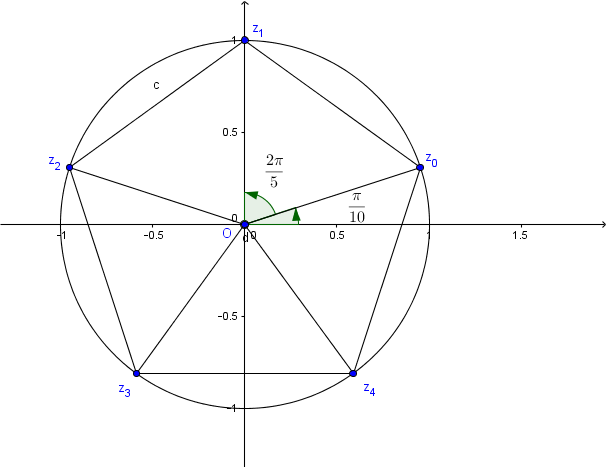
\includegraphics[scale=0.55]{images/202.png}
\caption{Racines $5^{iemes}$ de $z=e^{i\frac{\pi}{2}}=i$}
\end{center} \end{figure}

\subsubsection{Racines primitives de l'unité}
On appelle racine $n^{ieme}$ primitive de l'unité les $\omega \in \C$ tels que $\omega^{n}=1$ et $\forall$ $k \in \rrbracket 0;n-1 \rrbracket$, $\omega^{k}\neq 1$.

\begin{figure}[h] \begin{center}
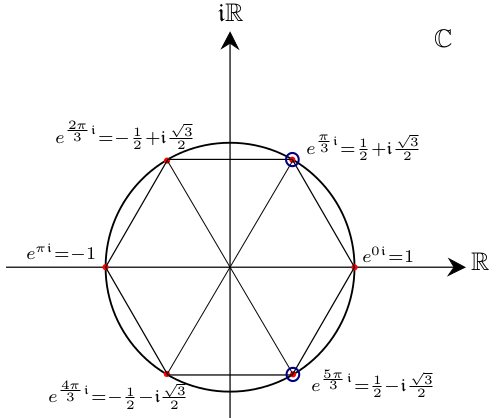
\includegraphics[scale=0.375]{images/204.png}
\caption{Racines $6^{iemes}$ de l'unité}
\emph{Les racines primitives sont entourées}
\end{center} \end{figure}

La somme des racines n$^{iemes}$ de l'unité est nulle.\\

\emph{Proposition : } soit $\omega$ une racine n$^{ieme}$ primitive de l'unité, alors l'ensemble des racines n$^{ieme}$ de l'unité est : $\{1$, $\omega$, $\omega^{2}$,..., $\omega^{n-1}\}$.

\subsubsection{Démonstration}
On veut montrer qu'il n'y a pas deux valeurs identiques dans la liste $\{1$, $\omega$, $\omega^{2}$,..., $\omega^{n-1}\}$.\\

\emph{Par l'absurde : } $\exists$ $(k,l) \in$ $\llbracket 0;n-1 \rrbracket^{2}$, avec $k\neq l$ mais $\omega^{k}=\omega^{l}$\\
L'un est plus petit que l'autre : $k<l$,\\ 
$\omega^{k}=\omega^{l-k} \Leftrightarrow  1=\omega^{l-k}$ donc $l=k$ car $(k,l) \in$ $\llbracket 0;n-1 \rrbracket^{2}$, ce qui est contradictoire.\\\\

On sait qu'il y a n racines qui sont les $\omega^{k}$ et que si $l\neq k$ alors $\omega^{k}\neq \omega^{l}$ car $(k,l) \in$ $\llbracket 0;n-1 \rrbracket^{2}$.\\

Alors $\{1$, $\omega$, $\omega^{2}$,..., $\omega^{n-1}\}$ est l'ensemble des racines n$^{ieme}$ de l'unité.

\subsection{Équations du $2^{nd}$ degré}
\subsubsection{Théorème}
Soient $(a; b; c) \in \C^{*}{}^{3}$, l'équation du second degré $az^{2}+bz+c=0$\\
admet $\left \{ \begin{array}{rcl} \text{2 solutions dans } \C &\text{ si }& b^{2}-4ac\neq 0\\ \text{1 solution dans } \C &\text{ si }& b^{2}-4ac=0 \end{array} \right .$\\\\\\
Lorsque $\delta$ satisfait $\delta^{2}=b^{2}-4ac\neq 0$, les solutions sont $\left \{ \begin{array}{rcl} z_{+}&=&\frac{-b+\delta}{2a} \\\\ z_{-}&=&\frac{-b-\delta}{2a} \end{array} \right . $\\

\subsubsection{Démonstration}
$\begin{array}{rcl} az^{2}+bz+c&=&a[(z+\frac{b}{2a})^{2}-(\frac{b^{2}-4ac}{4a^{2}})] \\ &=&a[(z+\frac{b}{2a})^{2}-(\frac{\delta}{2a})^{2}] \\\\ &=& a(z+\frac{b+\delta}{4a})(z+\frac{b-\delta}{4a}) \end{array}$

\newpage

\section{Formules}
\subsection{Formule de Moivre}
Une autre application de la représentation exponentielle est la formule de Moivre qui établit que
$cos(nx)+isin(nx)=[cos(x)+isin(x)]^{n}$
pour $n \in \Z$ et $x \in \R$.

\[cos(nx)+isin(nx)=\sum_{k=0}^{n} \dbinom{n}{k}cos(x)^{n-k} i^{k} sin(x)^{k}\]
\begin{center} (d'après la formule du binôme de Newton) \end{center}

En prenant la partie réelle:\\
\[cos(nx)=\sum_{0\leq k\leq \frac{n}{2}} \dbinom{n}{2k} cos(x)^{n-2k}(-1)^{k} sin(x)^{2k}\]
\[cos(nx)=\sum_{0\leq k\leq \frac{n}{2}} \dbinom{n}{2k} cos(x)^{n-2k}(-1)^{k} (1-cos(x)^{2})^{k}\]\\

Aussi on établi que le polynôme $T_{n}$ défini par $T_{n}(X)=\sum \limits_{0\leq k\leq \frac{n}{2}} (-1)^{k} \dbinom{n}{2k} X^{n-2k}(1-X^{2})^{k}$ qui satisfait $cos(nx)=T_{n}(cos(x))$ et est appelé polynôme de Tchebychev.\\\\
$T_{2}(X)=X^{2}-(1-X^{2})=2X^{2}-1$\\
$T_{3}(X)=X^{3}-3X(1-X^{2})=4X^{3}-3X$\\

Les $T_{2m}$ sont pairs et les $T_{2m+1}$ sont impairs.\\

\subsection{Formules d'Euler}
Les formules d'Euler établissent que $cos(x)=\frac{e^{ix}+e^{-ix}}{2}$ et $sin(x)=\frac{e^{ix}-e^{-ix}}{2i}$.\\

\textit{Avec le cosinus :}\\\\
$cos(x)^{2}=(\frac{e^{ix}+e^{-ix}}{2})^{2}=\frac{e^{2ix}}{4}+\frac{e^{-2ix}}{4}+\frac{1}{2}=\frac{1}{2}cos(2x)+\frac{1}{2}$\\\\
$cos(x)^{3}=(\frac{e^{ix}+e^{-ix}}{2})^{3}=\frac{e^{3ix}}{8}+\frac{e^{-3ix}}{8}+\frac{3}{4}(e^{ix}+e^{-ix})=\frac{1}{4}cos(3x)+\frac{3}{4}cos(x)$\\\\
$cos(x)^{4}=(\frac{e^{ix}+e^{-ix}}{2})^{4}=\frac{1}{8}cos(4x)+\frac{4}{8}cos(2x)+\frac{6}{16}=\frac{1}{8}cos(4x)+\frac{1}{2}cos(2x)+\frac{3}{8}$\\\\

\textit{Avec le sinus :}\\\\
$sin(x)^{2}=(\frac{e^{ix}-e^{-ix}}{2i})^{2}=-\frac{1}{4}(e^{2ix}+e^{-2ix}-2)=-\frac{1}{2}cos(2x)+\frac{1}{2}$\\\\
$sin(x)^{3}=(\frac{e^{ix}-e^{-ix}}{2i})^{3}=-\frac{1}{8i}(e^{3ix}+e^{-3ix}+3e^{ix}-3e^{-ix})=-\frac{1}{4}sin(3x)-\frac{3}{4}sin(x)$\\\\
$sin(x)^{4}=\frac{1}{8}(cos(4x)-4cos(2x)+3)$\\\\\\\\



\textit{Remarque : Une expression trigonométrique s'exprime en fonction de la tangente si elle est $\pi$ périodique.}
\newpage

\section{Géométrie et nombres complexes : les similitudes}
\subsection{Définition}
Une similitude est une application f du plan vers lui-même telle que pour tout points P et Q la distance $d(f(P),f(Q))=\lambda d(P,Q)$ où $\lambda \in \Rpe$ est une constante qui s'appelle le rapport de similitude de f.\\

Une similitude de rapport 1 est une isométrie.

\subsection{Théorème}
L'ensemble des similitudes est décrit par les transformations de $\C$ dans $\C$ données par\\
$f(z)=az+b$ ou $f(z)=a\overline{z}+b$ où $a \in \C ^{*}$ et $b \in \C$.\\

Ces transformations sont des isométries si et seulement si $|a|=1$.\\\\

\textbf{Démonstration :}\\\\
$f(z)=az+b$ ou $f(z)=a\overline{z}+b$ correspondent bien a des similitudes.\\

En effet, si $a=1$, il s'agit de la translation dont le vecteur a pour affixe $b$,\\
et si $a\neq 1$, le point $\Omega$ d'affixe $\omega =\frac{b}{1-a}$ est fixe et la transformation s'écrit $f(z)=ke^{i\theta }(z-\omega )+\omega$\\
(avec $k=|a|$ et $\theta =\arg(a)$).\\

Il s'agit donc de la composée de l'homothétie de centre $\Omega$ et de rapport k par la rotation de centre $\Omega$ et d'angle $\theta$.\\\\\\

On va maintenant montrer que toute similitude s'écrit sous la forme $f(z)=az+b$.\\

Soient O et A les points d'affixes respectives 0 et 1 ; O' et A' leurs images (distinctes) par cette transformation et b et c leurs affixes.\\

Soient $M\neq O$ un point quelconque d'affixe z, et M' son image d'affixe z'. Alors\\\\
\[ \frac{O'M'}{O'A'}=\frac {OM}{OA} \text{ et } (\overrightarrow {O'A'},\overrightarrow {O'M'})=(\overrightarrow {OA},{\overrightarrow {OM}}) \]

donc $\frac {z'-b}{c-b}=\frac {z-0}{1-0}=z$,\\\\
c'est-à-dire, en notant a le complexe $c-b$ (qui est non nul) : $z'=az+b$.\\\\\\

On peut noter que cette relation est vérifiée pour $M=O$, on a alors $M'=O'$ donc $b=a*0+b$.

\newpage

\subsection{Exemples} 
\begin{itemize}\renewcommand{\labelitemi}{$\bullet$}
\item \emph{La translation}\\

Soit $\vec{v}$ un vecteur dans le plan. La translation par $\vec{v}$ est la transformation qui associe à tout point P du plan l’unique point Q tel que $\overset{\longrightarrow}{PQ}=\vec{v}$.\\\\
Soit $b \in \C$ l’affixe du vecteur $\vec{v}$. Alors la translation par $\vec{v}$ correspond\\
à l’application $\tau_{b} : \begin{array}{rcl} \C &\longrightarrow &\C \\ z &\longmapsto &z + b \end{array}$\\\\

\item \emph{La rotation}\\

Soit C un point d’affixe $c \in \C$. La rotation de centre C et d’angle $\alpha$ est la transformation qui à tout point P du plan associe le point Q tel que $||CP||=||CQ||$ et $\widehat{PCQ}=\alpha$.\\

La rotation du plan de centre C et d’angle $\alpha \in [0;2\pi]$ correspond alors\\
à l’application $\rho_{c}, \alpha : \begin{array}{rcl} \C &\longrightarrow &\C \\ z &\longmapsto &e^{i\alpha} (z-c) + c = e^{i\alpha}z+(1-e^{i\alpha})c \end{array}$\\

Cette rotation transforme le repère $(O;\vec{i};\vec{j})$ en le repère orthonormal\\
$(M$ $;$ $\cos(\alpha)\vec{i}+\sin(\alpha)\vec{j}$ ; $\cos(\alpha)\vec{j}-\sin(\alpha)\vec{i})$, où M est le point d’affixe $(1-e^{i\alpha})c$.\\

Si $\alpha \equiv 0 (2\pi)$, c’est une translation et le centre C est le seul point invariant par la rotation.\\\\

\item \emph{La symétrie axiale}\\

Si l’application f est une symétrie axiale d’axe $\Delta$ qui passe par le point I et admet le vecteur $\vec{u}$ comme vecteur directeur associé, alors $z'=e^{i2\theta}(\overline{z}-\overline{z_{I}})+z_{I}$ où $\theta$ désigne une mesure de l’angle $(\vec{i};\vec{u})$.\\\\

\item \emph{La symétrie glissante}\\

Si l’application f est une symétrie glissante d’axe $\Delta$ qui passe par le point I et admet le vecteur $\vec{u}$ comme vecteur directeur associé, alors $z'=e^{2i\theta}(\overline{z}-\overline{z_{I}})+z_{I}+z_{\vec{u}}$ désigne une mesure de l’angle $(\vec{i};\vec{u})$.\\\\

\item \emph{Les homothéties}\\

Une homothétie est une similitude de la forme $z \longmapsto az+b$ avec $a \in \Rpe$.\\

L'homothétie de centre C et de rapport $\lambda$ est la transformation du plan complexe vers lui-même qui envoie tout point du plan P sur l'unique point Q tel que $\overset{\longrightarrow}{CQ}=\lambda\overset{\longrightarrow}{CP}$.\\

Elle correspond à l'application $h_{c,\lambda}$ : $\begin{array}{rcl} \C &\longrightarrow &\C \\ z &\longmapsto &\lambda(z-c)+c=\lambda z+(1-\lambda)c \end{array}$\\
avec c l'affixe de C.\\

Le centre de l'homothétie est le point invariant: $z_{0}=f(z_{0}) \Leftrightarrow z_{0}=a*z_{0}+b \Leftrightarrow z_{0}=\frac{b}{1-a}$.
\end{itemize} \newpage

\section{Cercle trigonométrique}
\label{Cercle trigo}
\begin{center} \begin{figure}[!h] 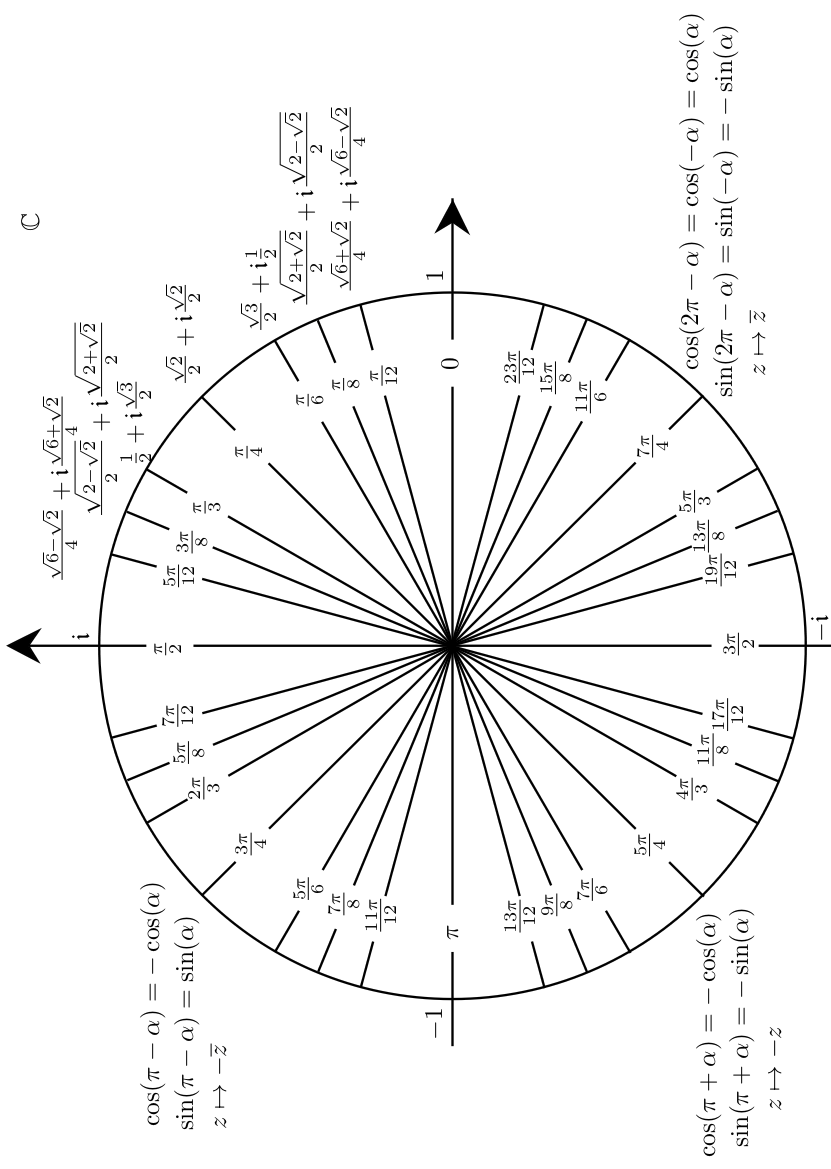
\includegraphics[scale=0.525]{images/205.png} \end{figure} \end{center}

\newpage

\includepdf[pages={51-87}]{images/CoursComplet.pdf}
\includepdf[pages={109-117}]{images/suite.pdf}

\end{document}